\documentclass[twoside]{article}
\usepackage{amsmath}
\usepackage{amssymb}
\usepackage{amsthm}
\usepackage{calc}
\usepackage{capt-of}
\usepackage{caption}
\usepackage[strict]{changepage}
\usepackage{chngcntr}
\usepackage[americanvoltage,siunitx]{circuitikz}
\usepackage{color,colortbl}
\usepackage{etoolbox}
\usepackage{fancyhdr}
\usepackage[T1]{fontenc}
\usepackage{gensymb}
\usepackage[margin=1in]{geometry}
\usepackage{graphicx}
\usepackage{hyperref}
\usepackage{import}
\usepackage{indentfirst}
\usepackage{mathptmx}
\usepackage{mathrsfs}
\usepackage{multicol}
\usepackage{multirow}
\usepackage{needspace}
\usepackage{pgfplots}
\usepackage{pgfplotstable}
\usepackage{setspace}
\usepackage{siunitx}
\usepackage{tabu}
\usepackage{tabularx}
\usepackage{tikz}
\usepackage{xspace}

\patchcmd{\thebibliography}{\section*{\refname}}{\vspace{-1em}}{}{}

\captionsetup{labelformat=empty,labelsep=none}
\usepgfplotslibrary{external}
\usetikzlibrary{positioning,matrix,shapes,chains,arrows}
\tikzexternalize[prefix=precompiled_figures/]

\newcommand\svgsize[2]{\def\svgwidth{#2}
{\centering\input{#1.pdf_tex}}}
\newcommand\svgc[1]{\svgsize{#1}{\columnwidth}}
\newcommand\svgl[1]{\svgsize{#1}{1em}}
\newcommand\diagrams[0]{\renewcommand\svgsize[2]{\def\svgwidth{##2}
{\centering\input{diagrams/##1.pdf_tex}}}}

\newcommand\pdf[1]{\noindent\includegraphics[width=\columnwidth]{#1.pdf}}
\newcommand\pdfex[1]{\pdf{#1}

\pdf{#1ex}}
\newcommand\pdfmsg[1]{\noindent\begin{minipage}{\columnwidth}\pdf{#1msg}

\pdf{#1}\end{minipage}}
\newcommand\pdfmsgex[1]{\pdfmsg{#1}

\pdf{#1ex}}
\newcommand\code[0]{\renewcommand\pdf[1]{\noindent
\includegraphics[width=\columnwidth]{code/##1.pdf}}}

% Indent
\setlength{\parindent}{0.3in}

\newcounter{paperthmamount}
\newcommand\theorems[0]{
\theoremstyle{remark}
\newtheorem{claim}[subsection]{Claim}
\theoremstyle{plain}
\newtheorem{conjecture}[subsection]{Conjecture}
\theoremstyle{plain}
\newtheorem{corollary}[subsection]{Corollary}
\theoremstyle{definition}
\newtheorem{definition}[subsection]{Definition}
\theoremstyle{plain}
\newtheorem{lemma}[subsection]{Lemma}
\theoremstyle{remark}
\newtheorem{proposition}[subsection]{Proposition}
\theoremstyle{remark}
\newtheorem{remark}[subsection]{Remark}
\theoremstyle{plain}
\newtheorem{theorem}[subsection]{Theorem}
\theoremstyle{definition}
\newtheorem{question}[subsection]{Question}
\newcommand\paperclm[2]
{\begin{claim}\global\expandafter\edef
\csname clm##1\endcsname{Claim \thesubsection\noexpand\xspace}
##2\end{claim}}
\newcommand\papercnj[2]
{\begin{conjecture}\global\expandafter\edef
\csname cnj##1\endcsname{Conjecture \thesubsection\noexpand\xspace}
##2\end{conjecture}}
\newcommand\papercor[2]
{\begin{corollary}\global\expandafter\edef
\csname cor##1\endcsname{Corollary \thesubsection\noexpand\xspace}
##2\end{corollary}}
\newcommand\paperdef[2]
{\begin{definition}\global\expandafter\edef
\csname def##1\endcsname{Definition \thesubsection\noexpand\xspace}
##2\end{definition}}
\newcommand\paperlem[2]
{\begin{lemma}\global\expandafter\edef
\csname lem##1\endcsname{Lemma \thesubsection\noexpand\xspace}
##2\end{lemma}}
\newcommand\paperprp[2]
{\begin{proposition}\global\expandafter\edef
\csname prp##1\endcsname{Proposition \thesubsection\noexpand\xspace}
##2\end{proposition}}
\newcommand\paperqtn[2]
{\begin{question}\global\expandafter\edef
\csname qtn##1\endcsname{Question \thesubsection\noexpand\xspace}
##2\end{question}}
\newcommand\paperrem[2]
{\begin{remark}\global\expandafter\edef
\csname rem##1\endcsname{Remark \thesubsection\noexpand\xspace}
##2\end{remark}}
\newcommand\paperthm[2]
{\begin{theorem}\global\expandafter\edef
\csname thm##1\endcsname{Theorem \thesubsection\noexpand\xspace}
##2\end{theorem}}}
\newcommand\subtheorems[0]{\stepcounter{paperthmamount}
\theoremstyle{remark}
\newtheorem{claim}[subsubsection]{Claim}
\theoremstyle{plain}
\newtheorem{conjecture}[subsubsection]{Conjecture}
\theoremstyle{plain}
\newtheorem{corollary}[subsubsection]{Corollary}
\theoremstyle{definition}
\newtheorem{definition}[subsubsection]{Definition}
\theoremstyle{plain}
\newtheorem{lemma}[subsubsection]{Lemma}
\theoremstyle{remark}
\newtheorem{proposition}[subsubsection]{Proposition}
\theoremstyle{remark}
\newtheorem{remark}[subsubsection]{Remark}
\theoremstyle{plain}
\newtheorem{theorem}[subsubsection]{Theorem}
\theoremstyle{definition}
\newtheorem{question}[subsubsection]{Question}
\newcommand\paperclm[2]
{\begin{claim}\global\expandafter\edef
\csname clm##1\endcsname{Claim \thesubsubsection\noexpand\xspace}
##2\end{claim}}
\newcommand\papercnj[2]
{\begin{conjecture}\global\expandafter\edef
\csname cnj##1\endcsname{Conjecture \thesubsubsection\noexpand\xspace}
##2\end{conjecture}}
\newcommand\papercor[2]
{\begin{corollary}\global\expandafter\edef
\csname cor##1\endcsname{Corollary \thesubsubsection\noexpand\xspace}
##2\end{corollary}}
\newcommand\paperdef[2]
{\begin{definition}\global\expandafter\edef
\csname def##1\endcsname{Definition \thesubsubsection\noexpand\xspace}
##2\end{definition}}
\newcommand\paperlem[2]
{\begin{lemma}\global\expandafter\edef
\csname lem##1\endcsname{Lemma \thesubsubsection\noexpand\xspace}
##2\end{lemma}}
\newcommand\paperprp[2]
{\begin{proposition}\global\expandafter\edef
\csname prp##1\endcsname{Proposition \thesubsubsection\noexpand\xspace}
##2\end{proposition}}
\newcommand\paperqtn[2]
{\begin{question}\global\expandafter\edef
\csname qtn##1\endcsname{Question \thesubsubsection\noexpand\xspace}
##2\end{question}}
\newcommand\paperrem[2]
{\begin{remark}\global\expandafter\edef
\csname rem##1\endcsname{Remark \thesubsubsection\noexpand\xspace}
##2\end{remark}}
\newcommand\paperthm[2]
{\begin{theorem}\global\expandafter\edef
\csname thm##1\endcsname{Theorem \thesubsubsection\noexpand\xspace}
##2\end{theorem}}}

% Title section
\pagestyle{fancy}
\thispagestyle{empty}
\renewcommand{\headrulewidth}{0pt}
\newcommand\papertitle[1]
{{\centering\fontsize{20pt}{20pt}\textsc{#1}\\\mbox{}\\}
\fancyhead[OC]{\fontsize{12pt}{12pt}\selectfont\textit{#1}}}
\newcounter{people}
\newcommand\paperauthtext[3]{{\centering\fontsize{12pt}{12pt}\selectfont
\textsc{#1}\\[-0.1em]{\fontsize{9pt}{9pt}\selectfont\textit{\ifx&#2&
\vspace{-1em}\else#2\fi}}\\\mbox{}\\
\fancyhead[EC]{\fontsize{12pt}{12pt}\selectfont\textit{#3}}}}
\newcommand\paperauth[2]{{\stepcounter{people}
\ifnum\value{people}=1
{\paperauthtext{#1}{#2}{#1}
\global\def\auth{#1\xspace}}
\else\ifnum\value{people}=2
{\paperauthtext{#1}{#2}{\auth and #1}}
\else{\paperauthtext{#1}{#2}{\auth et al}}\fi\fi}}
\newcommand\physics[0]{
\renewcommand\paperauthtext[4]{{\centering\fontsize{12pt}{12pt}\selectfont
\textsc{##1. ##2}\\[-0.1em]{\fontsize{9pt}{9pt}\selectfont\textit{\ifx&##3&
\vspace{-1em}\else##3\fi}}\\\mbox{}\\
\fancyhead[EC]{\fontsize{12pt}{12pt}\selectfont\textit{##4}}}}
\renewcommand\paperauth[3]{{\stepcounter{people}
\ifnum\value{people}=1
{\paperauthtext{##1}{##2}{##3}{##1. ##2}
\global\def\auth{##2\xspace}}
\else\ifnum\value{people}=2
{\paperauthtext{##1}{##2}{##3}{\auth and ##2}}
\else{\paperauthtext{##1}{##2}{##3}{\auth et al}}\fi\fi}}}
\newcommand\paperdate[1]{{\centering\fontsize{9pt}{9pt}\selectfont\text{
(Received #1)}\\[2em]}}

% Page header
\newcommand{\paperhead}[1]{\fancyhead[EC]{\fontsize{12pt}{12pt}\selectfont
\textit{#1}}}
\fancyhead[RO, EL]{\fontsize{12pt}{12pt}\selectfont\thepage}
\fancyhead[RE, OL]{}
\cfoot{}

\makeatletter
\newenvironment{paperadjustwidth}[2]{
  \begin{list}{}{
    \setlength\partopsep\z@
    \setlength\topsep\z@
    \setlength\listparindent\parindent
    \setlength\parsep\parskip
    \@ifmtarg{#1}{\setlength{\leftmargin}{\z@}}
                 {\setlength{\leftmargin}{#1}}
    \@ifmtarg{#2}{\setlength{\rightmargin}{\z@}}
                 {\setlength{\rightmargin}{#2}}
    }
    \item[]}{\end{list}}
\makeatother

%Figure counter
\newcounter{paperfigurecounter}
\newcommand{\papercap}[2]{\bgroup\stepcounter{paperfigurecounter}
\captionof{figure}{\fontsize{9pt}{9pt}\selectfont
\hspace{0.3in}Fig.~\arabic{paperfigurecounter}.\quad#2}
\egroup\expandafter\edef
\csname fig#1\endcsname{Fig.~\arabic{paperfigurecounter}\noexpand\xspace}}

\newcommand\paperfig[3]{\noindent\begin{minipage}{\columnwidth}
#2\papercap{#1}{#3}\end{minipage}\expandafter\edef
\csname fig#1\endcsname{Fig.~\arabic{paperfigurecounter}\noexpand\xspace}}
\newcommand\papersvg[3]{\paperfig{#1}{\svgc{#2}}{#3}}

% Abstract environment
\newenvironment{paperabs}
{\begin{paperadjustwidth}{0.5in}{0.5in}\bgroup\fontsize{9pt}{9pt}\selectfont
\hspace{0.5in}}
{\egroup\end{paperadjustwidth}}

% Paper environment
\setlength\columnsep{0.5in}
\newenvironment{paper}
{\begin{multicols*}{2}\bgroup\fontsize{12pt}{12pt}\selectfont}
{\egroup\end{multicols*}}
\newcommand{\singlecolumn}[0]{
\renewcommand\paperfig[3]{\noindent
\makebox[\textwidth][c]{\begin{minipage}{5.5in}
\noindent\makebox[\textwidth][c]{\begin{minipage}{3in}##2\end{minipage}}
\papercap{##1}{##3}\end{minipage}}\expandafter\edef
\csname fig##1\endcsname{Fig.~\arabic{paperfigurecounter}\noexpand\xspace}}
\renewenvironment{paper}{\bgroup\fontsize{12pt}{12pt}\selectfont}
{\egroup}}

%Sources
\newsavebox{\sourcebox}
\newcommand{\papersource}[1]{
\vspace{-2em}
\text{}\\*
\fontsize{9pt}{9pt}\selectfont
\noindent\renewcommand{\labelenumi}{}
\savebox{\sourcebox}{\parbox{3in}{\begin{enumerate}
\setlength{\leftmargini}{-1ex}
\setlength{\leftmargin}{-1ex}
\setlength{\labelwidth}{0pt}
\setlength{\labelsep}{0pt}
\setlength{\listparindent}{0pt}
\item\textit{\hspace{-0.35in}#1}
\end{enumerate}}}
\usebox{\sourcebox}
}

%Section headers
\newcounter{paperseccounter}
\newcounter{papersubseccounter}[paperseccounter]
\newcommand\papersec[1]{\needspace{1in}
\stepcounter{paperseccounter}
\stepcounter{section}
\begin{center}\Roman{paperseccounter} \textsc{#1}\end{center}}
\newcommand\papersubsec[1]{\needspace{1in}
\stepcounter{papersubseccounter}
\addtocounter{subsection}{\thepaperthmamount}
\setcounter{subsubsection}{0}
{\begin{center}
\Roman{section}.\Roman{papersubseccounter}
\textsc{#1}\\[0.5em]\end{center}}}

%equation
\newcounter{papereqcounter}
\newcommand\papereq[3]{{
\stepcounter{papereqcounter}
\mbox{}\vspace{-0.75em}
\begin{equation*}
#2
\tag*{\fontsize{12pt}{12pt}\selectfont
$\begin{array}{r}
\cr{\text{(\arabic{papereqcounter})}}
\cr{\fontsize{9pt}{9pt}\selectfont\textit{\ifx\\#3\\~\else(\fi#3\ifx\\#3\\~
\else)\fi}}
\end{array}$}
\end{equation*}

}
\expandafter\edef\csname eq#1\endcsname{(\arabic{papereqcounter})\noexpand
\xspace}}

% Where
\newcommand{\papervar}[3]
{&$#1$ & #2 \ifx\\#3\\~\else($\smash{\text{\si{\fi
#3\ifx\\#3\\~\else}}}$)\fi\\}
\newenvironment{paperwhere}
{\begin{minipage}{\columnwidth}
\bgroup\fontsize{9pt}{9pt}\selectfont Where:\vspace{2pt}\\\begin{tabular}
{rr@{ = }p{\linewidth}}}
{\end{tabular}\egroup\end{minipage}\vspace{5pt}}

% Tables
\definecolor{LineGray}{gray}{0.5}
\newtabulinestyle{outer=2.25pt LineGray}
\newtabulinestyle{inner=0.75pt LineGray}
\tabulinesep=1.5pt

\newcommand{\paperiline}[0]{\tabucline[inner]{-}}
\newcommand{\paperoline}[0]{\tabucline[outer]{-}}

% Index column type
\newcolumntype{I}{X[-5,c]}
% Column type with uncertainty
\newcolumntype{U}{@{}X[-5,r]@{$\pm$}X[-5,l]@{}}
% Column type without uncertainty
\newcolumntype{C}{@{}X[-5,c]@{}}

\newcounter{papertableindexcounter}
\newcommand{\papertableindexheader}[0]{\multirow{2}{*}{\textsc{Index}}}
\newcommand{\papertableindex}[0]{\stepcounter{papertableindexcounter}
\arabic{papertableindexcounter}}
\newcommand{\papertableuheadersymbol}[1]{&\multicolumn{2}{c|[inner]}{$#1$}}
\newcommand{\papertableuheadersymbole}[1]{&\multicolumn{2}{c|[outer]}{$#1$}}
\newcommand{\papertableuheaderunit}[1]{&\multicolumn{2}{c|[inner]}{(#1)}}
\newcommand{\papertableuheaderunite}[1]{&\multicolumn{2}{c|[outer]}{(#1)}}
\newcommand{\papertablecheadersymbol}[1]{&$#1$}
\newcommand{\papertablecheaderunit}[2]{&($\pm$#1 #2)}

% Value in table with uncertainty.
\newcommand{\papertableuval}[2]{& #1 & #2}
% Value in table without uncertainty.
\newcommand{\papertablecval}[1]{& #1}

\newenvironment{papertable}[1]
{\setcounter{papertableindexcounter}{0} 
\begin{tabu} to \linewidth {#1}}
{\end{tabu}\vspace{12pt}}

\newcommand{\paperaxis}[9]
{title=#1,
axis x line = bottom,
xmin=#4,xmax=#6,
axis y line = left,
ymin=#5,ymax=#7,
height = 180pt,
grid=both,
x axis line style=-,
y axis line style=-,
x tick label style={
/pgf/number format/.cd,
fixed,
fixed zerofill,
precision=#8,
/tikz/.cd},
y tick label style={
/pgf/number format/.cd,
fixed,
fixed zerofill,
precision=#9,
/tikz/.cd}}
\newcommand{\paperaxisxlabel}[2]{
xlabel=\fontsize{10pt}{10pt}\selectfont#1$(#2)\rightarrow$}
\newcommand{\paperaxisylabel}[2]{
ylabel=\fontsize{10pt}{10pt}\selectfont#1$(#2)\rightarrow$}
\newcommand{\papergraphoutline}[4]{
\addplot [mark=none,line width=0.75pt] coordinates {
(#1,#2)
(#1,#4)
(#3,#4)
(#3,#2)
(#1,#2)};}

\newenvironment{papergraph}{
\begin{tikzpicture}
\begin{axis}}
{\end{axis}
\end{tikzpicture}}

\newcommand{\comment}[1]{}

\newcommand{\abs}[1]{\left\lvert#1\right\rvert}
\newcommand{\oo}[0]{\infty}
\newcommand{\sigmaSum}[3]{\sum\limits_{#1}^{#2} #3}
\newcommand{\limto}[3]{\lim\limits_{#1\rightarrow#2}#3}
\renewcommand{\d}[0]{\mathrm{d}}
\newcommand{\cross}[0]{\times}
\newcommand{\lp}{\left(}
\newcommand{\rp}{\right)}
\newcommand\pars[1]{\lp#1\rp}
\newcommand\sqbrack[1]{\left[#1\right]}
\newcommand\R{\mathbb{R}}
\newcommand\di{\partial}
\newcommand\x{\times}
\newcommand\del{\nabla}

\physics
\begin{document}
\papertitle{Analysis of the Constantan Thermocouple}
\paperauth{A}{Khesin}{1002442029}
\paperauth{N}{Rahnamaei}{1002552686}
\paperauth{P}{Zavyalova}{1002345036}
\paperdate{January 24, 2018}
\begin{paperabs}
	
	In this experiment the EMF across a thermocouple was measured at a variety of temperatures to investigate the Seebeck Effect. Plotting the obtained data on a calibration curve proved the expected linear relationship. Upon fitting the temperature differences to the potential using the least squares method, the Seebeck coefficient was determined to be \( \pars{41.0 \pm .3} \si{\micro\volt\per\kelvin} \). Further, the resistance of the thermocouple was measured to be $(1.8\pm.4)\si{\ohm}$.
	
\end{paperabs}

\begin{paper}
	
\papersec{Introduction}

	Thermocouples convert a temperature difference into an electromotive force (EMF), and are made of two wires of dissimilar metals which are joined at each end. The wires in a temperature gradient will allow the free carriers at the hot end have more kinetic energy and tend to diffuse towards the cold end, which will in turn create an electric field which has a averse tendency the heat flow. In this experiment, the temperature difference was established between an ice bath staying at constant temperature, and another body of water with varying temperature. 
	
	EMF generated along the conductor is quantified by the Seebeck Effect, a proportionality law relating the potential and the temperature difference.
	\papereq{Seebeck}{V = S\pars{T_1 - T_2}}{Serbanescu}
	\begin{paperwhere}
		\papervar{V}{potential difference}{\volt}
		\papervar{S}{Seebeck coefficient}{\volt\per\kelvin}
		\papervar{T_1}{absolute temperature at first junction}{\kelvin}
		\papervar{T_2}{absolute temperature at second junction}{\kelvin}
	\end{paperwhere}
	
	This equation is convenient as it is linear in both temperature difference and potential.
	Temperatures were measured in degrees Celsius and compared to freezing, so they were equal to the temperature differences.
	
	The experiment setup included a voltmeter, two thermal flasks to ensure that the temperature was kept constant and a thermometer all arranged as shown below.
	
	\paperfig{setup}{\centering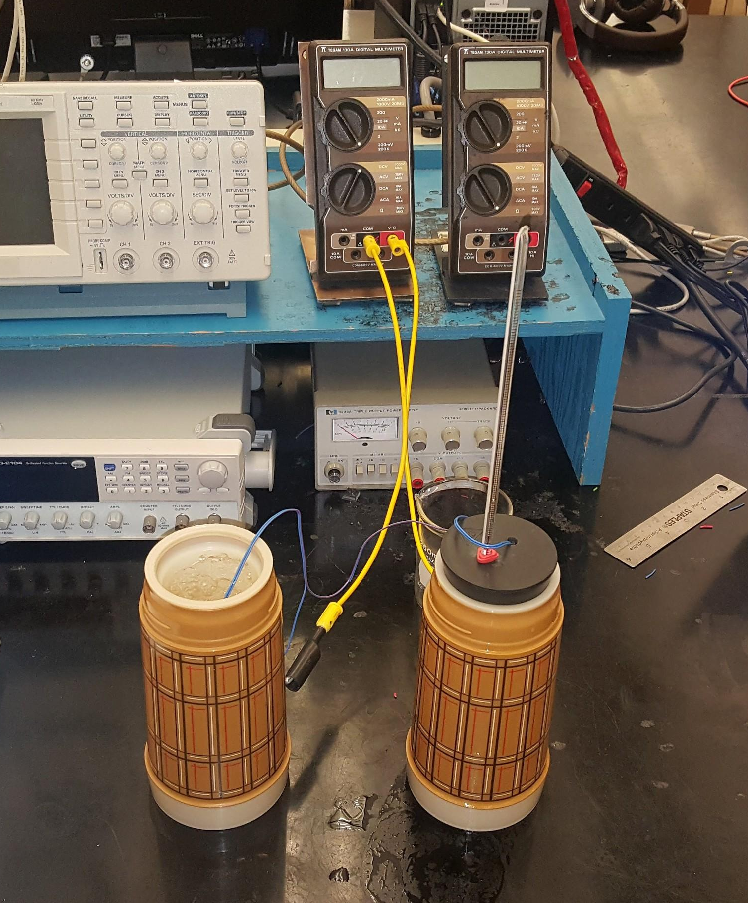
\includegraphics[width=0.9\columnwidth]{setup.pdf}}{The setup of the experiment.}	
	
	The circuit used in the experiment was as follows.
	
	\paperfig{Circuit}{\center
	\begin{tikzpicture}[scale=0.7,transform shape]
	\draw (1,0) to[voltmeter] (3,0) -- (3,1) -- (4,1) -- (4,2) -- (5,2)
	(4,2) -- (4,3) -- (0,3) -- (0,2) -- (-1,2) -- (0,2) -- (0,1) -- (1,1) -- (1,0);
	\draw (0.3,1.5) node[right]{$B$};
	\draw (3.3,1.5) node[right]{$B$};
	\draw (1.8,2.5) node[right]{$A$};
	\draw (-1,2) node[left]{$T_1$};
	\draw (5,2) node[right]{$T_2$};
	\end{tikzpicture}
	}{The circuit diagram used in the experiment.
	The wire marked $A$ was made of Constantan and the wires marked $B$ were made of Copper.
	The temperature difference was being measured between points $T_1$ and $T_2$.
	The voltmeter shown at the bottom was used to measure the potential differences in the circuit.}	
	
\papersec{Observations}
	
	The temperature $T_1$ in the ice water bath was kept at a constant $(0.0\pm.5)\degree C$.
	This value was occasionally remeasured during the experiment to make sure that it was unchanged.
	The recorded values for the temperatures at $T_2$ and for the potential differences $V$ were recorded in the table below.
	
	\paperfig{Table}{\centering\scalebox{0.9}[0.9]{\begin{papertable}{|[outer]I|[inner]C|[inner]C|[outer]}\paperoline
	\papertableindexheader&\multirow{2}{*}{\textsc{Temperature}\vspace{0.5em}}&\multirow{2}{*}{\textsc{Potential}\vspace{0.5em}}\\
	\papertablecheadersymbol{T_2$ ($\si{\celsius}$) $(\pm.5\si{\celsius})}\papertablecheadersymbol{V$ ($\si{\volt}$) $(\pm.1\si{\volt})}\\\paperiline
	\papertableindex\papertablecval{97.0}\papertablecval{4.0}\\\paperiline
	\papertableindex\papertablecval{79.5}\papertablecval{3.3}\\\paperiline
	\papertableindex\papertablecval{70.0}\papertablecval{2.9}\\\paperiline
	\papertableindex\papertablecval{60.0}\papertablecval{2.4}\\\paperiline
	\papertableindex\papertablecval{46.5}\papertablecval{1.9}\\\paperiline
	\papertableindex\papertablecval{38.5}\papertablecval{1.5}\\\paperiline
	\papertableindex\papertablecval{30.0}\papertablecval{1.2}\\\paperiline
	\papertableindex\papertablecval{24.5}\papertablecval{1.0}\\\paperiline
	\papertableindex\papertablecval{17.0}\papertablecval{0.7}\\\paperiline
	\papertableindex\papertablecval{9.5}\papertablecval{0.3}\\\paperiline
	\papertableindex\papertablecval{3.0}\papertablecval{0.1}\\\paperiline
	\papertableindex\papertablecval{0.0}\papertablecval{0.0}\\\paperoline
	\end{papertable}}\vspace{-0.5em}}{The observations recorded during the experiment of the relationship between $T_2$ and $V$.
	The value of $T_1$ was not included in the table as it was constant.}
		
\papersec{Analysis} 
	
	To calibrate the thermocouple, measured EMF values were plotted against the temperature difference between the junctions. Upon fitting the data using least squares method, the Seebeck coefficient was determined to be \( \pars{41.0 \pm .3} \si{\milli\volt\per\kelvin} \). The value of reduced \( \chi ^2 \) for this fit was \( 0.202632 \). The calibration curve, fit, and residuals are visualized below. 
	
	\paperfig{CalibrationCurve}{\pdf{ThermocoupleCalibration}}{EMF and residuals plotted against the temperature difference between the junctions. The curve has the function \(  \pars{0.041.0 \pm 0.000.3} \Delta T \) and an \( R^2 \) value of \( 0.998821 \).}\columnbreak
	
	In this experiment, the output resistance of the thermocouple was measured.
	The value of this resistance was calculated to be $(1.8\pm.4)\si{\ohm}$.

	The precision of any measurements made in this experiment could have been increased by using several thermocouples in series.
	Since the differences in temperature between the endpoints of the thermocouples would have added up to the difference between the first and last endpoint, this would have measured the same value of temperature difference, but the fact that the temperature would be measured in many smaller pieces would increase the precision of the measurement.
	The situation would be identical if a large distance more precisely by measuring many smaller intervals which together add to the longer distance.
	Thus, there would be a advantage to connecting several thermocouples in series.
	
\papersec{Conclusion}

	The experiment investigated the Seebeck Effect.
	Although the goodness of the obtained fit was quite high, the experiment was not free from sources of error.
	In spite of the fact that the ice water bath temperature was occasionally measured, its temperature might have fluctuated during the experiment.
	Furthermore, the construction and connections in the actual thermocouple itself could have been less than ideal.
	
	The Seebeck coefficient was determined to be \( \pars{41.0 \pm .3} \si{\micro\volt\per\kelvin} \), close the value for Constantan, -35. Note that the sign of the coefficient is not relevant as it is obtained by flipping the poles of the voltmeter. Further, the resistance of the thermocouple was measured to be $(1.8\pm.4)\si{\ohm}$.

\papersec{Sources}

	\papersource{Serbanescu, R., The Thermocouple, 2013}

\end{paper}

\end{document}